\section{Introduction}

Understanding the past climate of the earth allows for us to begin to understand what effects we are having upon it, and to predict what the future will bring.
From the analysis of isotope ratios in ice cores and marine sediment cores, we obtain knowledge of past temperature from the ratio of $\delta ^{18} O$, a proxy for combined temperature and global ice volume.
This time series is constructed over the past 2 Myr, with higher values indicating a colder climate as the ocean is enriched with $\delta ^{18} O$ during the colder conditions.
The variation in the orbital parameters of our planet affect the amount of solar insolation recieved, and the timescale variation of these quantities is one possible forcing for past climatic change.
This was hypothesized as early as the nineteenth century, and further elucidated by Milankovitch, whose name the study of these variations bears.
The eccentricity of our eliptical orbit is changing slowly in time, as is the orientation of the planet's spin axis and the longitude closest to the sun at the vernal equinox.
We refer to these parameters as $e$, $\epsilon$ and $\overline{\omega}$, respectively.

The main questions arising about this time period from Dijkstra \cite{dijkstra2013} that any satisfactory theory of the Pleistocene Ice Ages should explain are:
\begin{itemize}
\item Why did the glacial-interglacial cycles appear in the Pleistocene?
\item Which processes in the climate system caused the glacial-interglacial changes in global mean temperature, $p^a_{CO_2}$, and ice sheet extent?
\item What caused the transistion (the MPT) from the 41-kyr world to the 100-kyr world about 700 kyr ago?
\end{itemize}

\begin{figure}[tpb!]
\centering
  \includegraphics[width=.48\textwidth]{../data/dO18/d18O_lisiecki_noname.pdf}
  \caption{
    The LR04 benthic $\delta ^{18} O$ stack over the Pleistocene, constructed by the graphic correlation of fifty-seven globally distributed benthic $\delta ^{18} O$ records versus time (data from Lisieki \cite{lisiecki2005pliocene}).
  }
  \label{fig:insol-data}
\end{figure}

The Milankovitch theory of orbital forcing is now the `null hypothesis' answer to these questions, and various models are available that relate this orbital forcing to global mean temperature and ice sheet extent have been proposed.
The fit between the changing solar insolation and $\delta ^{18} O$ has been demonstrated not to be linear, opening the door for more complex explanations.
The potentially impoortant feedbacks of ice-albedo, height-mass balance, load-accumulation, and precipation-temperature have all been combined into quasi-equilibrium and internal oscillation models, with the latter successfully demonstrating a reasonable fit to the data.
In addition to these more complex models is a switching equilibria model from Didier Paillard that fits the data emprically, and does ``remarkable'' considering the simplicity of the model.

In the present work we attempt a rigorous fit of Paillard's model to data using the tools of evolutionary computation.

\begin{figure}[tpb!]
\centering
  \includegraphics[width=.45\textwidth]{../src/discrete_plot_noname.pdf}
  \caption{
    The discrete Paillard model.
  }
  \label{fig:paillard-fig3}
\end{figure}

\section{Paillard's Model}

With some difficulty understanding his original paper \cite{paillard1998timing}, we recontruct Paillard's model for both versions that he provides.
The following two subsections paraphrase \cite{paillard1998timing} directly.

\subsection{Discrete model}

\newcommand{\inter}{\textbf{i}}
\newcommand{\mild}{\textbf{g}}
\newcommand{\full}{\textbf{G}}

The model has three states called \inter~(interglacial), \mild~(mild glacial) and \full~(full glacial).
This model undergoes an \inter-\mild~transistion as soon as the insolation falls below $i_0$.
An \mild-\full~transistion happens when the ice volume exceeds a threshold $v_\text{max}$ and finally a transistion \full-\inter~occurs when the insolation increases above $i_1$.
These transistions are assumed to be one-way, and the only ones allowed are those just discussed.
The \mild-\full~transition has the constraints that it will happen after some time $t_g$ and with insolation lower than some level $i_3$.
If $t_g$ is exceeded but $i_3$ is also exceeded, then the \mild-\full~transistion occurs as the next insolation decrease: when insolation falls below $i_2$.
% THIS MODEL IS WEIRDDDDDD

The part which was made least clear was whether the insolation exceeding $i_3$ necessitates a reset of the time in state \mild until $t_g$ is reached.
To achieve similar results, we assume that the answer is yes, the time does reset.



\subsection{Differential equation model}


This model is an extension of the discrete model.
There are still three regimes but now we define the ice volume $v$ as a differential equation

$$ \frac{dv}{dt} = (v_R - v) /\tau _R - F/\tau _F .$$

where $R$ is the current climate regime ($R$ = \inter,\mild,\full), $v_R$ are the reference ice volumes for the different regimes, $F$ is the forcing and $\tau _{R,F}$ are the time constants.
The transistions are the same for \inter-\mild~and \full-\mild~but \mild-\full~now happens when $v \geq v_\text{max}$, some threshold value (without any condition on the insolation).
Paillard also ``normalizes the ice volume to unity'': $v_g = v_G = v_\text{max} = 1$ and $v_i = 0$.
For the finale of model weirdness, the forcing $F$ is defined as a truncated insolation signal with truncation function $f$ as

$$ f(x) = \frac{1}{2} \left ( x + \sqrt{4a^2 + x^2} \right ) $$

and setting $a=1$.

\section{Computing Insolation}

The only input to the model is the solar insolation, so we are particulary careful to obtain accurate values.
Increasingly accurate integrations of the state of the solar system have been performed dating from the time of Lagrange in 1781 through Milankovich's use of Pilgrim's 1904 computations to establish his theory of past climate change to today's direct numerical integrations \cite{laskar2004long}.

Using the orbital parameters of eccentricity $e$, obliquity $\epsilon$, and longitude of the parahelion $\overline{\omega}$ computed from an integration function insola.f provided from Laskar \cite{laskar2004long} we can reconstruct the insolation at any time.
The following derivation is due to Berger \cite{berger1981long}.

The insolation $Q$ at a given location and time can be written as a function of the solar constant $S_0$, the distance from the Earth to sun relative to the average $R_0/R_E$ the solar zenith angle $\Theta$:

$$ Q = S_0 \frac{R_0^2}{R_E^2} \cos (\Theta) .$$

To solve for the average insolation during one day at a given latitute $\phi$, we need to express the solar zenith angle $\Theta$ in terms of $\phi$ and the known orbital parameters.
Taking $\delta$ as the latitude of the point directly subsolar and $h$ as the hour angle, we use the spherical law of cosines to write

$$ \cos ( \Theta ) = \sin ( \phi ) \sin ( \delta ) + \cos ( \phi ) \cos ( \delta ) \cos ( h ) .$$

Now to have the average daily insolation $\overline{Q} _\text{day}$ we take the integral of $Q$ from $h_o $ to $-h_0$ where $h_0$ is the hour angle for which the sun first rises.
Since we are concerned with the $\phi = $65N, the sun always rises and sets so we won't consider the cases for the sun neither rising nor setting.
Integrating, we have

$$ \overline{Q} _\text{day} = \frac{S_0}{\pi } \frac{R_0^2}{R_E^2} \left [ h_0 \sin (\phi) \sin (\delta) + \cos (\phi) \cos (\delta) \sin (h_0) \right ] . $$

Defining $\theta = 0$ the be the vernal equinox, we can write $\delta$ and $R_0/R_E$ as a function of the orbital parameters in a simple form at the summer solsctice ($\theta = \pi /2$):

$$ \delta = \epsilon ~~~~\text{and} ~~~~ \frac{R_0}{R_E} = 1 + e\sin (\overline {\omega}) .$$

\begin{figure}[tpb!]
\centering
  \includegraphics[width=.48\textwidth]{../data/insolation/laskar2004/insol_data2_noname.pdf}
  \caption{
    The average daily solar insolation $\overline{Q}_{\text{day}}$ is computed on the summer solstice at 65N with the prodived $e,\epsilon,$ and $\overline{\omega}$.
  }
  \label{fig:insol-data}
\end{figure}


\section{Evolutionary Algorithm Methods}

\newcommand{\bb}[1]{\mathbb{#1}}
\newcommand{\DO}{$\delta^{18}O$ }

We attempt to search the parameter space within the limits suggested by Paillard \cite{paillard1998timing} in hopes of better fitting the both the discrete and the ODEE models to the \DO data by using a genetic algorithm (GA) and covariance matrix adaption evolutionary scheme (CMA-ES) to evolve possible parameters. CMA-ES and GA are well-known and documented evolutionary algorithms for evolving real-valued vectors that minimize a particular fitness function when evaluated.
For this investigation, we chose to minimize the root mean square error of the normalized model compared to the \DO data.

\subsection{Datasets for fitting}
We obtained to necessary data sets for running our experiments.
Our \DO data comes from Tiedermann et al. \cite{d18} as the result of analyzing San ice core sample taken from up to 273.80 m in 1986. A simple linear transformation is used to scale from depth to the age of the samples. The ice core sample was taken in the North Atlantic Ocean. While this may not be the exact dataset used by Paillard, we believe the data contained here should be sufficiently similar and relevant in our efforts to fit Paillard's models to historical climate behavior.\\
\indent We employ the same insolation dataset used by Paillard in \cite{paillard1998timing}; namely, we use the data provided by A. Berger in \cite{berger1981long}.
Berger obtains this curve representing the earth's atmospheric insulation about the latitude $65^{o}N$ by modeling the earth's rotation about the sun.
His calculations account for such variables as the angle of the earth's axis from perpendicular to the sun, and eccentricity.
This insolation curve acts as the forcing for our model.

\subsection{Models in more detail}
Paillard \cite{paillard1998timing} suggests two models for obtaining the \DO curves from atmospheric insolation data. These models represent the transformations of three different glacial states: $i$ (interglacial), $g$ (mild glacial), $G$ (full glacial). Both models allow us to impose limits on the insolation, the ice volume that determines the glacial state, and the expected time spent in each glacial state. In both models, it is assumed that the only three possible transitions exists. A $i\rightarrow g$ (interglacial$\rightarrow$ mild glacial) transition occurs when when the insolation falls below a parameter $i_{0}$. A $g\rightarrow G$ (mild glacial $\rightarrow$ full glacial) transition occurs when a maximum ice volume $v_{max}$ is exceeded. Finally, a $G\rightarrow i$ (full glacial$\rightarrow$ interglacial) transition occurs when the insolation grows above a parameter.

Paillard first suggests a discrete model for obtaining the \DO curve from insolation data. This model has four insolation parameters.  $i_{0}$ and $i_{1}$ represent the insolation values required for $i-g$ and $G-i$ transitions to occur, respectively. The other insolation parameters $i_{2}$ and $i_{3}$ identify a range of possible forcing values that would allow a $g-G$ transition to occur. A further parameter, $\tau_{g}$, is a time constant determining the minimum number of years for the model to spend in a mild glacial state. In an effort to reduce the search space, we adopt Paillard's assumption of $\tau_{g}=33$ kyr for our discrete model and attempt to evolve values for the parameters $i_{0}$, $i_{1}$, $i_{2}$, and $i_{3}$.

An ODE model is also presented by Paillard, which is given by \[ \frac{dv}{dt}=\frac{v_{R}-v}{\tau_{R}}-\frac{F}{\tau_{F}} \] where $v$ is the ice volume, $v_{R}$ and $\tau_{R}$ are the volume and the time constants, respectively, corresponding to the glacial state. $\tau_{F}$ is a time constant associated with a forcing parameter $F$. The forcing parameter $F$ is given through a truncation of the insolation data described by \[ F=\frac{1}{2}(x+\sqrt{4a^{2}+x^{2}})\] with $x$ being the insolation and a tunable compression parameter $a$. $i_{0}$ and $i_{1}$ are the same as in the discrete model, and the other insolation parameters are omitted. Again, we reduce our search space by adopting the assumption presented by Paillard that $\tau_{i}=10$ kyr, $\tau_{g}=\tau_{G}=50$ kyr, $\tau_{F}=25$ kyr, and $a=1$. We attempt to provide good choices for the remaining insolation parameters $i_{0}$ and $i_{1}$.\\

\subsection{Evolutionary Algorithms}
Both of the evolutionary algorithms we used are designed to search through the space $\bb{R}^{n}$ with a population of $n$ length real-valued vectors with each entry corresponding to a parameter in our model. Through common genetic mechanisms, like reproduction and mutation, we are able to evolve vectors representing potentially good parameter choices for the insolation parameters in each model to fit the \DO  data. Both algorithms require a fitness function with which to assess how well the parameter choices represented by an individual vector represent the \DO data through the models. We employ a fitness function which integrates the model and then attempts to minimize the root mean square error of the resulting time series compared to the true \DO data. This fitness function allows us to apply selection pressure on the populations of vectors that results in competition within the population to fit the \DO data the best.\\
\vspace{.25cm}

\noindent{\bf Covariance Matrix Adaption Evolutionary Scheme (CMA-ES)}\\
CMA-ES is often a good initial choice of evolutionary algorithm for evolving real-valued vectors because the algorithm itself is not expensive and the algorithm often yields a reasonably good result after only a few generations. The algorithm begins with a uniformly distributed cloud of points in $\bb{R}^{n}$. Each point represents parameter choices for the models. We asses the fitness of each point and create a covariance matrix weighted by the fitness values. By taking the average of the fitness values, we can determine weighted center of the cloud of points, and we can determine a direction to move that point that will hopefully yield a better average fitness. Having relocated the average point, we create a new cloud of points around the average, however we now use the covariance matrix to determine how to distribute the individuals points. For example, if the population members all agree at a particular index, then they will have small covariances. This will cause the new cloud of points to be very narrow in that dimension since all of the population members are in agreement. On the other hand, if all of the individuals disagree in a particular dimension, then there will be large covariances representing a need to explore more in that dimension. Thus, the cloud of points should be wider in that dimension. We fix the number of generations to be 500 for our experiments. More information about CMA-ES can be found in \cite{suttorp}.

\begin{figure}[tpb!]
\centering
  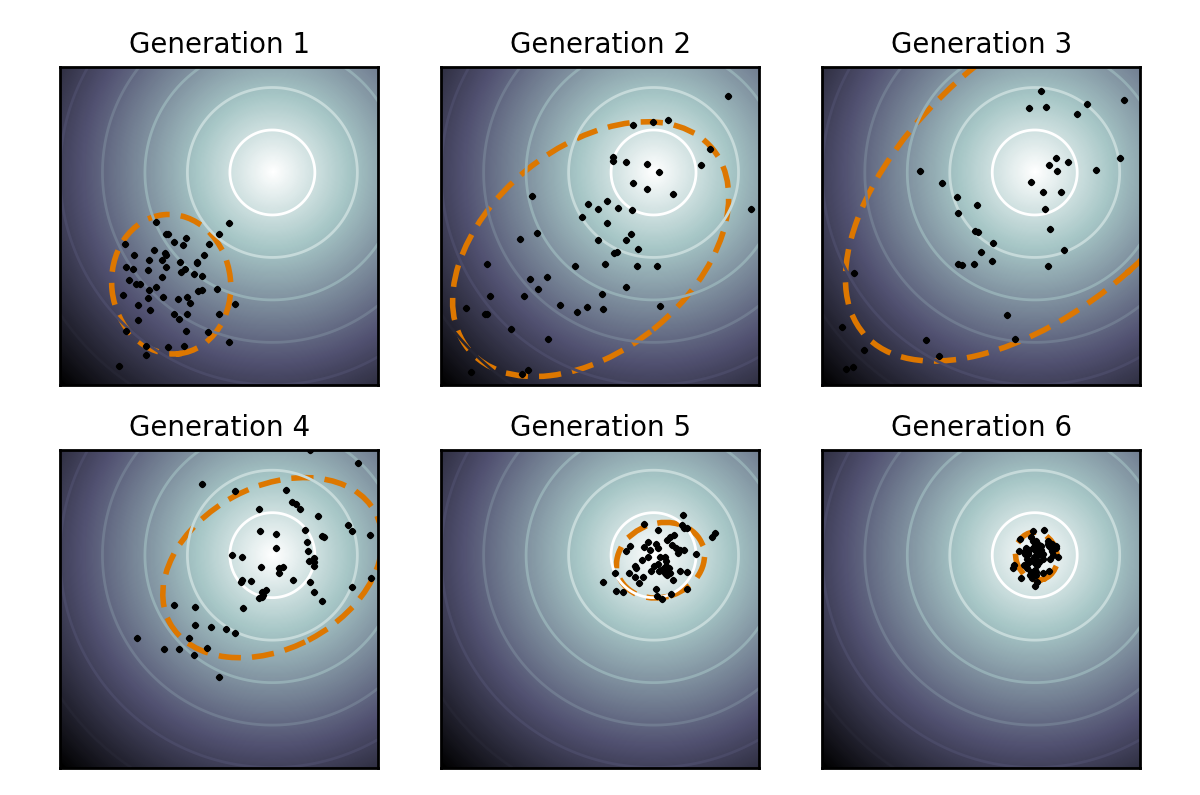
\includegraphics[width=.48\textwidth]{cmaes.png}
  \caption{
    A cartoon representing 6 generations in a CMA-ES experiment. Here, lighter colors indicate improved fitness. The dashed lines represent the influence of the covariance matrix.\\
    }
  \label{fig:cmaes}
\end{figure}


\noindent{\bf Genetic Algorithm (GA)}\\
GA's are typically more expensive than CMA-ES, but allow for an increased wealth in ways for population members to combine information. GA's often yield greater runtimes than CMA-ES but can also yield more robust explorations of parameter space. The algorithm begins with a population of real-valued vectors. Each vector is assessed for fitness. The fitter individuals in the population are chosen as candidates for reproduction in the form of crossover. Here, we use uniform crossover, which means that given two ``parent" vectors from the population, we create a ``child" vector by randomly selecting indices to contain the value stored in that index by parent 1. The remaining indices are filled with the values stored in parent 2 at those indices. A second child vector is created by taking the same random indices, and swapping the roles of the parents. These two children vectors then replace their parents in the population. Individuals in the population are also subject to mutation. Mutation is performed on individuals where a small amount is added or subtracted from each index in an individual vector with some small probability. Crossover often leads the population to converge on good solutions, while mutation generally causes the population to explore parameter space. Striking a balance between these two forces is vital and often very difficult depending on the noise in the fitness landscape; that is, the fitness values associated with each point in the parameter space. For our experiments, we use a population size of 500 and calculate 500 generations.

\begin{figure}[tpb!]
\centering
  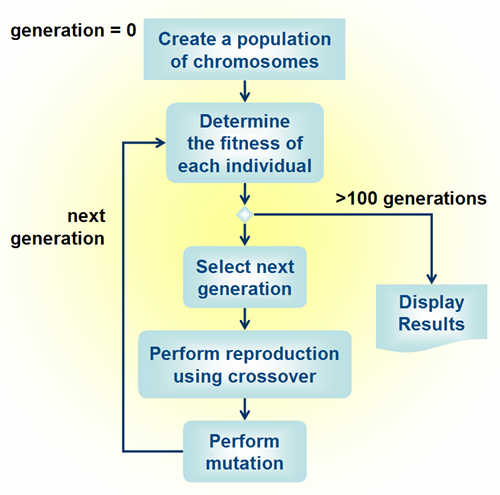
\includegraphics[width=.48\textwidth]{gaImg.png}
  \caption{
      A schematic explaining the basic steps in a genetic algorithm.
    }
  \label{fig:ga}
\end{figure}

\section{Results}

Constructin the insolation from orbital parameters, Figure \ref{fig:insol-data} depicts the reconstruction of insolation data back in time from Laskar's data set. And verifying that our interpretation of the model is the same as Paillard intended, Figure \ref{fig:paillard-fig3} is a direct representation of the second figure of Paillard's original paper \cite{paillard1998timing}.

Having run 100 CMA-ES and GA experiments, we discuss the fit of the best solutions here. Firstly, CMA-ES underperformed. None of the CMA-ES experiments yielded results worth noting here. This is likely due to unresolvable noise in the fitness landscape. We focus instead on the more promising results from our GA experiments.

\begin{figure}[tpb!]
\centering
  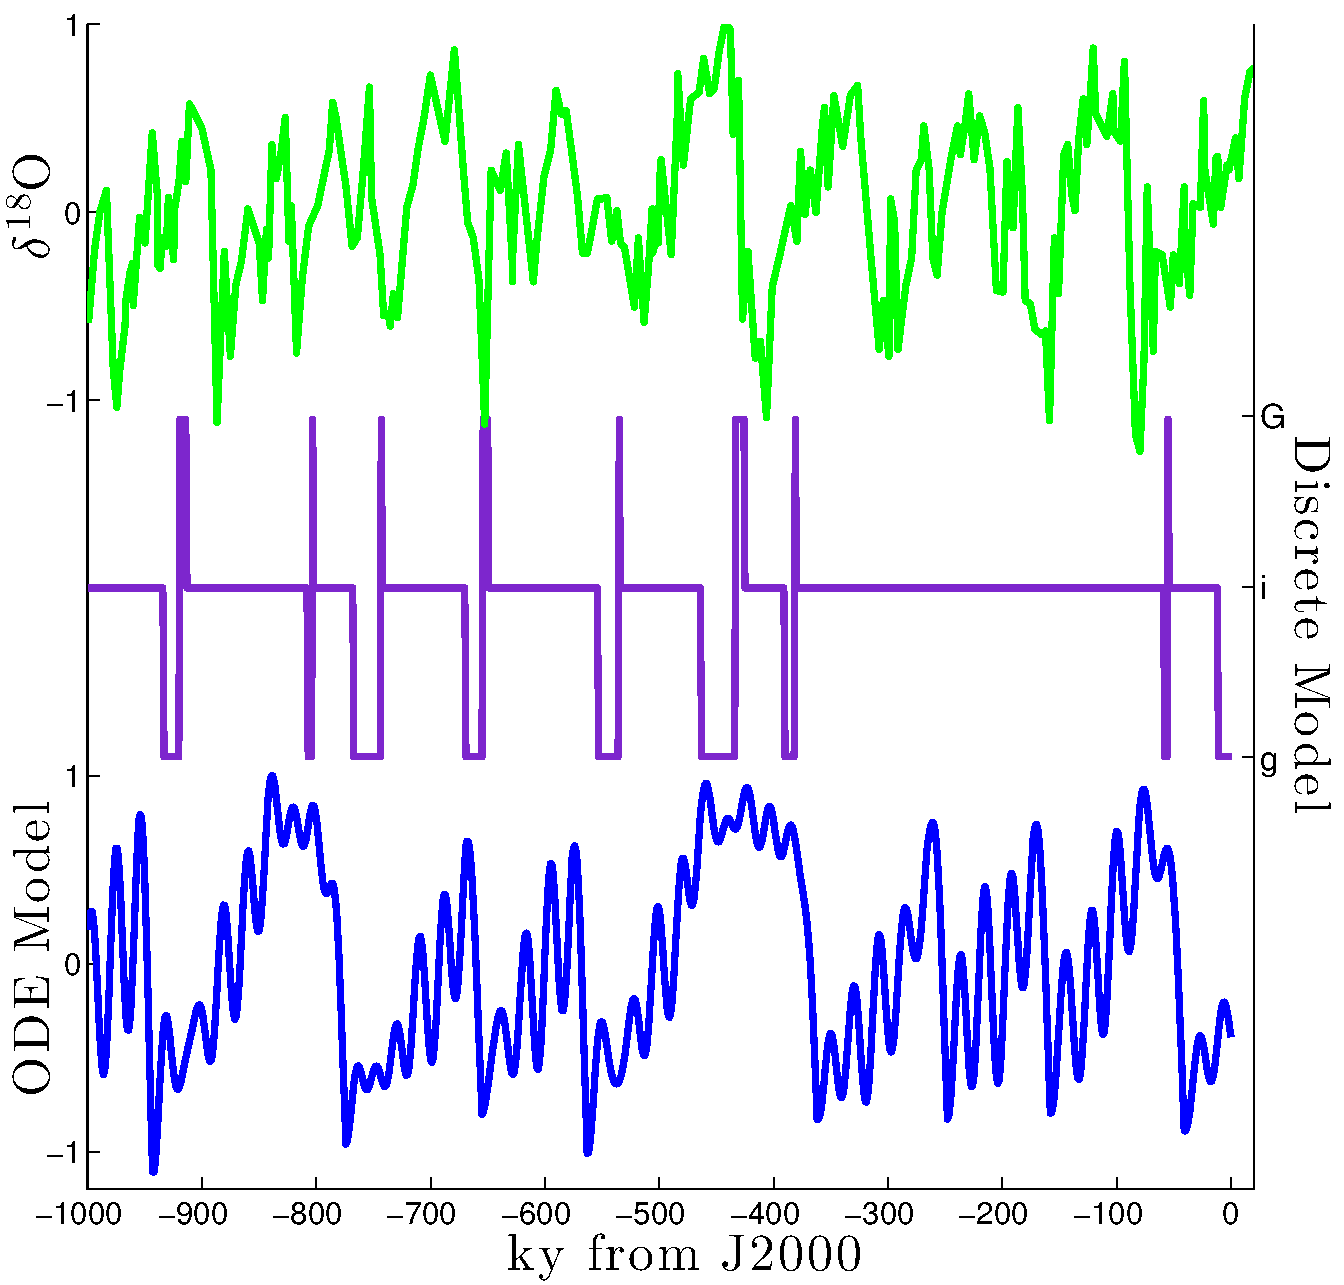
\includegraphics[width=.48\textwidth]{../src/results_plot_noname.pdf}
  \caption{
      The best result from the GA experiments attempting to fit parameters to Paillard's discrete and ODE model, with the \DO data used for fitness.
    }
  \label{fig:results}
\end{figure}

Figure \ref{fig:results} demonstrates the results of our most promising GA experiments along with their root mean square errors (RMSE) from the \DO data. We should note that the particular parameter choices proposed by Paillard in \cite{paillard1998timing} yield RMSE$=1.42$ for the discrete model, and RMSE$=1.7186$ for the ODE model. Figure 3 shows that our GA experiment ($i_{0}= -0.7293$, $i_{1}=-0.2287$, $i_{2}=0.0803$, and $i_{3}=0.9862$) was only narrowly outperformed by Paillard's parameter choices for the discrete model, and that our GA experiment ($i_{0}= -0.9677$ and $i_{1}=0.0294$) yields a better fitting ODE model than the model suggested by Paillard's parameter choices for this model.

\section{Conclusion}

The fitted Paillard model of climatic variability makes a strong case for differing atmospheric states playing a role in the temperature variation in the $\delta ^{18} O$ record.
The methods of evolutionary computation are important in climate science to assist in model validation, an important step in understanding.
With only forcing from changing solar insolation, this verifies that past climatic varaition of larger time scales is a result of the variation of the Earth's orbital parameters.



